\documentclass[12pt]{article}
\usepackage{amsfonts,amsthm,amsmath,amssymb,mathtools}
\usepackage{mathrsfs}
\usepackage{enumitem}
\usepackage{tikz-cd}
\usepackage{geometry}
\usepackage{mlmodern}
\usepackage{graphicx}

\geometry{letterpaper, portrait, margin=1in}

\setcounter{section}{0}

\renewcommand{\thesection}{\S\arabic{section}}
\renewcommand{\thesubsection}{\arabic{section}}
\DeclareMathOperator{\im}{im}
\DeclareMathOperator{\id}{id}

\newtheorem{thm}{Theorem}
\newenvironment{theorem}[1]{
	\renewcommand{\thethm}{#1}
	\begin{thm}
		}{\end{thm}}

\newtheorem{lma}{Lemma}
\newenvironment{lemma}[1]{
	\renewcommand{\thelma}{#1}
	\begin{lma}
		}{\end{lma}}

\theoremstyle{definition}
\newtheorem{ex}{Assignment}
\newenvironment{exercise}[1]{
	\renewcommand{\theex}{#1}
	\begin{ex}
		}{\end{ex}}

\title{MTH 732 Topology - Homework 7}
\author{Connor Mooneyhan}
\date{March 5, 2026}

\begin{document}

\maketitle

\begin{ex}
	Consider the following 3-simplex, which we denote by $[v_0, v_1, v_2, v_3]$.\\
	\begin{center}
		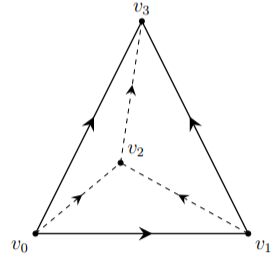
\includegraphics[width=0.3\textwidth]{3-simplex}\\
	\end{center}
	We compute its boundary and label its faces as follows: \begin{equation*}
		\partial[v_0, v_1, v_2, v_3] = \underbrace{[v_1, v_2, v_3]}_\text{A} - \underbrace{[v_0, v_2, v_3]}_\text{B} + \underbrace{[v_0, v_1, v_3]}_\text{C} - \underbrace{[v_0, v_1, v_2]}_\text{D}.
	\end{equation*}
	Let $X$ be the space resulting from gluing faces $A$ to $B$ and $C$ to $D$.
	Compute the simplicial homology groups $H^\Delta_n(X)$.
	\textit{Hint: there should be one 3-simplex, two 2-simplices, three 1-simplices, and two 0-simplices.}
	What space is this?
\end{ex}
\begin{proof}
  Here's my attempt at a picture:
	\begin{center}
		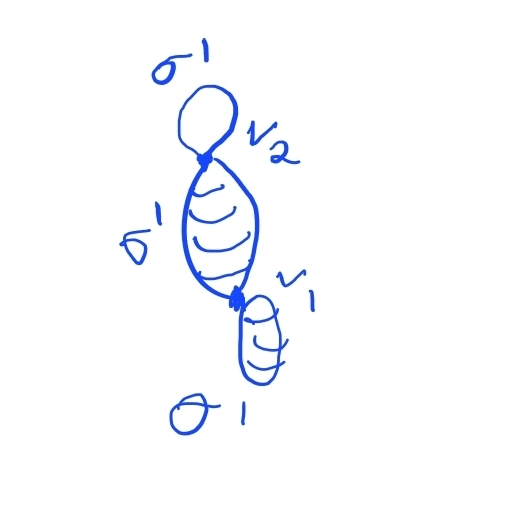
\includegraphics[width=0.3\textwidth]{complex}\\
	\end{center}
	\begin{itemize}
		\item The 0-simplices are $[v_1]$ and $[v_2]$.
		      Thus $\ker\partial_0 = \mathbb{Z}\left\langle [v_1], [v_2] \right\rangle$.
		\item The 1-simplices are $[v_1, v_1]$, $[v_1, v_2]$, and $[v_2, v_2]$.
		      Thus $\ker\partial_1 = \mathbb{Z}\left\langle [v_1, v_1], [v_2, v_2] \right\rangle$ and $\im\partial_1 = \mathbb{Z}\langle[v_2 - v_1]\rangle$.
		\item The 2-simplices are $[v_1, v_1, v_1]$ and $[v_1, v_2, v_2]$.
		      Thus $\partial_2[v_1, v_1, v_1] = [v_1, v_1]$, and $\partial_2[v_1, v_2, v_2] = [v_2, v_2]$, so $\ker\partial_2 = 0$ and $\im\partial_2 = \mathbb{Z}\langle[v_1, v_1], [v_2, v_2]\rangle$.
		\item The 3-simplex is $[v_1, v_1, v_2, v_2]$, so $\partial_3  = 0$.
	\end{itemize}
	Since there are no 4-simplices whose boundaries we can mod out by, we immediately get $H_3^\Delta(X) \cong \mathbb{Z}$.
  We also immediately get $H_2^\Delta(X) \cong 0$ since $\ker\partial_2 = 0$.
  We now get $H_1^\Delta(X) = \mathbb{Z}\left\langle [v_1, v_1], [v_2, v_2] \right\rangle/ \mathbb{Z}\left\langle [v_1, v_1], [v_2, v_2] \right\rangle \cong 0$.
  Finally, we have $H_0^\Delta(X) = \mathbb{Z}\left\langle [v_1], [v_2] \right\rangle/\mathbb{Z}\left\langle [v_2 - v_1] \right\rangle \cong \mathbb{Z}$.

  My guess for what this space was was $S^1 \vee S^2 \vee S^2$. 
  Visually, that's what it looks like, but the homology doesn't match up, so I'm not sure what I would call this.
\end{proof}

\begin{ex}
	Are there group homomorphisms $f$ and $g$ such that \begin{equation*}
		\begin{tikzcd}[column sep=small]
			0 \arrow[r] & \mathbb{Z}_4 \arrow[r, "f"] & \mathbb{Z}_8 \oplus \mathbb{Z}_2 \arrow[r, "g"] & \mathbb{Z}_4 \to 0
		\end{tikzcd}
	\end{equation*}
	is a short exact sequence?
\end{ex}
\begin{proof}
	Define \begin{align*}
		f & : 1 \mapsto (2, 1) \\ g & : (x, y) \mapsto x + 2y.
	\end{align*}
	Then $f$ is injective as required since \begin{align*}
		f(1) & = (2, 1) \\
		f(2) & = (4, 0) \\
		f(3) & = (6, 1) \\
		f(0) & = (0, 0)
	\end{align*}
	and $g$ is surjective as required since \begin{align*}
		g(0, 0) & = 0  \\
		g(1, 0) & = 1  \\
		g(0, 1) & = 2  \\
		g(1, 1) & = 3.
	\end{align*}
	The other requirement for exactness is that $\im f = \ker g$.
	Indeed, on the image of $f$ as listed above, $g = 0$, and if $(x, y)$ were any other element of $\mathbb{Z}_8 \oplus \mathbb{Z}_2$, we would have $x$ being ``odd'', and since $2y$ is always ``even'', we could not end up with $x + 2y = 0$, so $\ker g = \im f$, and the sequence is exact.
\end{proof}

\begin{ex}
	Let \begin{equation*}
		\begin{tikzcd}[column sep=small]
			A \arrow[r, "f"] & B \arrow[r] & C \arrow[r] & D \arrow[r, "g"] & E
		\end{tikzcd}
	\end{equation*}
	be an exact sequence.
	Show that $C = 0$ (trivial group) if and only if $f$ is surjective \textbf{and} $g$ is injective.
\end{ex}
\begin{proof}
	We put a couple extra labels on the diagram like so: \begin{equation*}
		\begin{tikzcd}[column sep=small]
			A \arrow[r, "f"] & B \arrow[r, "\phi"] & C \arrow[r, "\psi"] & D \arrow[r, "g"] & E
		\end{tikzcd}.
	\end{equation*}
	If $C = 0$, then $\im f = \ker \phi = B$ and $\ker g = \im \psi = 0$.
	Thus $f$ is surjective and $g$ is injective as desired.

	If we first have $f$ being surjective and $g$ being injective, then we know that $\ker\phi = \im f = B$ and $\im \psi = \ker g = 0$.
	This forces $f$ to be the trivial map since $B$ is the kernel, so $\ker\psi = \im\phi = 0$, meaning $\psi$ is injective.
	Since $\im \psi = 0$, we conclude that $C$ has only one element and is thus the trivial group, as desired.
\end{proof}

\end{document}
